\chapter{Installazione ed utilizzo}

Tutto il codice sorgente è pubblico e disponibile nella \href{https://github.com/TendTo/EW-DER-Simulator}{repository di GitHub} \footnote{https://github.com/TendTo/EW-DER-Simulator}.
È possible consultare le Github action per trovare una versione eseguibile del simulatore per tutti i maggiori sistemi operativi. \\
Tuttavia, è consigliabile seguire la procedura descritta nella sezione seguente per compilare una propria versione del simulatore da sorgente.

\section{Download ed installazione delle dipendenze}

Il primo passo è clonare la repository o scaricare il sorgente come cartella compressa. \\
Dopo aver estratto tutto, il primo passo fondamentale è quello di installare le dipendenze indicate nel file \textit{package.json} con il comando \mintinline{bash}{npm install}.
Successivamente, è necessario compilare gli smart contract con \mintinline{bash}{npm run compile}. \\
Così facendo verranno prodotti anche i file di typing necessari all'applicativo scritto in typescript. \\
\\
Opzionalmente, se si ha intenzione di effettuare il deploy dello \gls{smart-contract} sulla \gls{blockchain},
bisogna creare un file \textit{.env} nella cartella \textit{contracts} ed inserire i dati necessari:
\begin{itemize}
    \item \textbf{VOLTA\_SK}=chiave segreta associata all'account che si vuole utilizzare
    \item \textbf{VOLTA\_NODE\_URL}=indirizzo ip del nodo \gls{rpc-api}
\end{itemize}
Una volta inseriti i dati, si può lanciare il comando \mintinline{bash}{npm run deploy:volta} iniziare il deploy.
Potrebbe essere necessario attendere un po' di tempo. \\
\\
Per lanciare il simulatore, è sufficiente eseguire il comando \mintinline{bash}{npm start}.

\section{Utilizzo del simulatore}

Prima di lanciare una simulazione, è possibile impostare i parametri che verranno utilizzati da quest'ultima dal pannello a sinistra (\autoref{fig:simulator}). \\
Per evitare dover inserire molte volte gli stessi parametri,
è possibile creare un file \textit{.env} nella cartella \textit{simulator} ed inserire i dati parametri utilizzati di frequente. \\
L'ordine di priorità nell'applicazione di un parametro è:
$$
    \text{pannello a sinistra} > \text{file .env} > \text{parametro di default}
$$
\\
Se si tratta del primo avvio, o si intendo utilizzare un numero maggiore di IoT, è necessario fornire loro dei fondi,
altrimenti non saranno in grado di invocare i metodi dello \gls{smart-contract}.
Una volta avviata la simulazione, potrebbe essere necessario attendere un po' di tempo per il reset dello \gls{smart-contract} e l'invio dei fondi ai \gls{der}. \\
Se il setup si è concluso con successo, pian piano compariranno gli \gls{event-log} che i \gls{der} hanno generato registrando gli \gls{agreement}.
Inoltre, sul grafico inizierà a comparire la lettura aggregata fornita dall'\gls{aggregator}. \\
\\
Per avviare una richiesta di flessibilità, è sufficiente indicare un valore nell'input in alto a destra e cliccare sul pulsante. \\
Il grafico verrà resettato per mostrare più chiaramente l'andamento della flessibilità, e l'\gls{aggregator} invierà la richiesta.
Non appena i \gls{der} la riceveranno, varieranno la loro produzione. \\
Il resoconto della flessibilità sarà prodotto alla conclusione di quest'ultima, al raggiungimento della terza riga verticale.

\begin{figure}[h]
    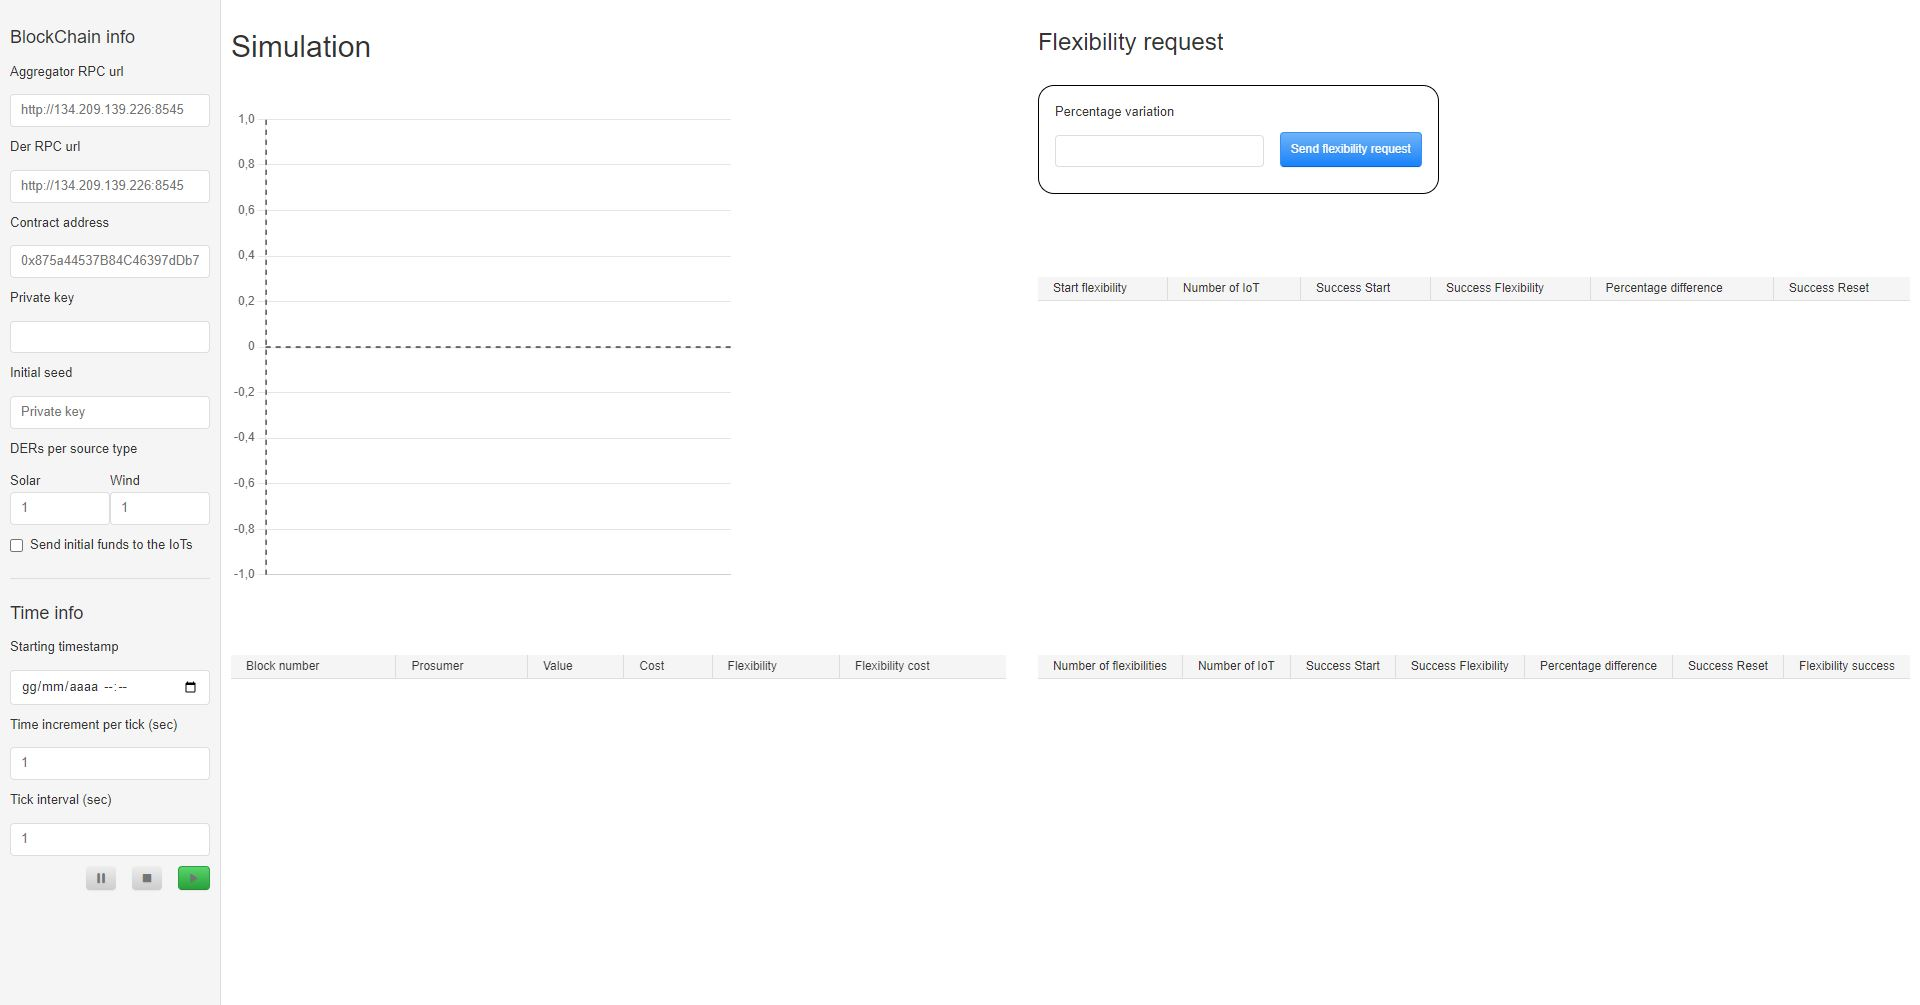
\includegraphics[width=\textwidth]{img/Simulator.jpg}
    \caption{Schermata del simulatore appena avviato \label{fig:simulator}}
\end{figure}

\section{Logging}

Al fine di poter avere un'idea chiara del comportamento del simulatore e poter notare eventuali errori,
è stato integrato un sistema di logging capillare.
I log con livello di priorità \textit{INFO} o superiore sono stampati sulla console,
ma è possibile consultare i log integrali o quelli specifici ad un certo componente dalla cartella \textit{simulator/logs}. \\
Per visualizzare l'andamento delle varie simulazioni, è particolarmente indicativo consultare il file \textit{simulator/logs/flexibility.log}. \\

Ogni riga conterrà i dati inerenti alla flessibilità nel formato:
\begin{center}
    {\scriptsize
        \texttt{blockNumber,numberOfIoT,percentageSuccessStart,percentageSuccessFlexibility,percentageSuccessReset,\\
        percentageDifferenceFromObjective,success}
    }
\end{center}
